\documentclass[a4paper, 11pt]{article}

%% Language and font encodings
\usepackage[T1]{fontenc}
\usepackage[utf8x]{inputenc}
\usepackage[english]{babel}


\usepackage[sfdefault,lf]{carlito}
%% The 'lf' option for lining figures
%% The 'sfdefault' option to make the base font sans serif
\usepackage[parfill]{parskip}
\usepackage{framed}
%\renewcommand*\oldstylenums[1]{\carlitoOsF #1}
\usepackage{fancyhdr}
\usepackage{authblk}
\setlength{\headheight}{41pt}
\usepackage[a4paper,top=3cm,bottom=2cm,left=2cm,right=2.5cm,marginparwidth=1.75cm]{geometry}
\usepackage[unicode=true,pdfusetitle,bookmarks=true,bookmarksnumbered=false,bookmarksopen=false,breaklinks=false,pdfborder={0 0 0},backref=false,colorlinks=true,allcolors=magenta]{hyperref}
%% Sets page size and margins



%\usepackage[left=1.5cm, right=2.5cm, marginparwidth=3.5cm, top=2.5cm, bottom=2.5cm]{geometry}
\usepackage{tabularx}
\usepackage{multirow}
\usepackage{booktabs}
\usepackage{caption}
\usepackage{subcaption}
\usepackage{enumerate}
\usepackage{mathtools, physics}
\usepackage{graphicx}
\setcounter{secnumdepth}{3}
\usepackage{amsmath}
\usepackage{amsthm}
\usepackage{amssymb}
\usepackage{mathrsfs}
\usepackage{enumerate}
\usepackage[textsize=small]{todonotes}
\presetkeys{todonotes}{color=yellow!20}{}
\newcommand{\CZ}{\mathit{CZ}}
\newcommand{\Ket}[1]{\ket{#1}} %adapt syntax of the braket package to the one of the physics package
\newcommand{\ksq}{\Ket{{}\mathop{\square}{}}}
\newcommand{\sq}{{}\mathop{\square}{}}%spaces to be like ×
%next needed because empty still takes room for missing indices
\NewDocumentCommand{\decosq}{O{} O{} O{} O{}}%
%        {\Ket{{\scriptstyle{#4}}\overset{#1}{\underset{#3}{\square}}{\scriptstyle{#2}}}}
        {{\scriptstyle{#4}}%
         \smashoperator{\mathop\square\limits^{#1}_{#3}}%
        {\scriptstyle{#2}}}
\NewDocumentCommand{\decoksq}{O{} O{} O{} O{}}%
         {\Ket{\decosq[#1][#2][#3][#4]}}
\newcommand{\fred}[2][]{\todo[color=red!30, #1]{\textbf{FG:} #2}}
%\newcommand{\kX}{\Ket{\times}}
\NewDocumentCommand{\kX}{O{} O{}}{\Ket{\prescript{#1}{#2}\times}}
\NewDocumentCommand{\mX}{O{} O{}}{\prescript{#1}{#2}\times}
\usepackage{colortbl}
\newcommand{\cm}[1]{\textcolor{blue}{#1}}
\newcommand{\intg}{\mathrm{d}}
\newcommand{\e}{\mathrm{e}}

%% Useful packages





%\renewcommand{\headrulewidth}{0pt}
\pagestyle{plain}
\title{Exercice 2}
\author{}

\begin{document}
\maketitle
\section{La première [3pt; 1pt pour la décomposition en cylindre, 2pt pour le résultat]}
Le cylindre est un objet formidable (observez la figure \ref{fig:cyl} si vous ne me croyez pas), surtout lorsqu'il a un rayon R et une hauteur h. La valeur de son volume va vous étonner ! Calculez-la en utilisant une intégrale simple. (Pour ce faire, vous vous rappelerez, avec nostalgie, l'équation d'un cercle de rayon R : $x^2+y^2=R^2$).

\begin{centering}

\begin{figure}
    \centering
    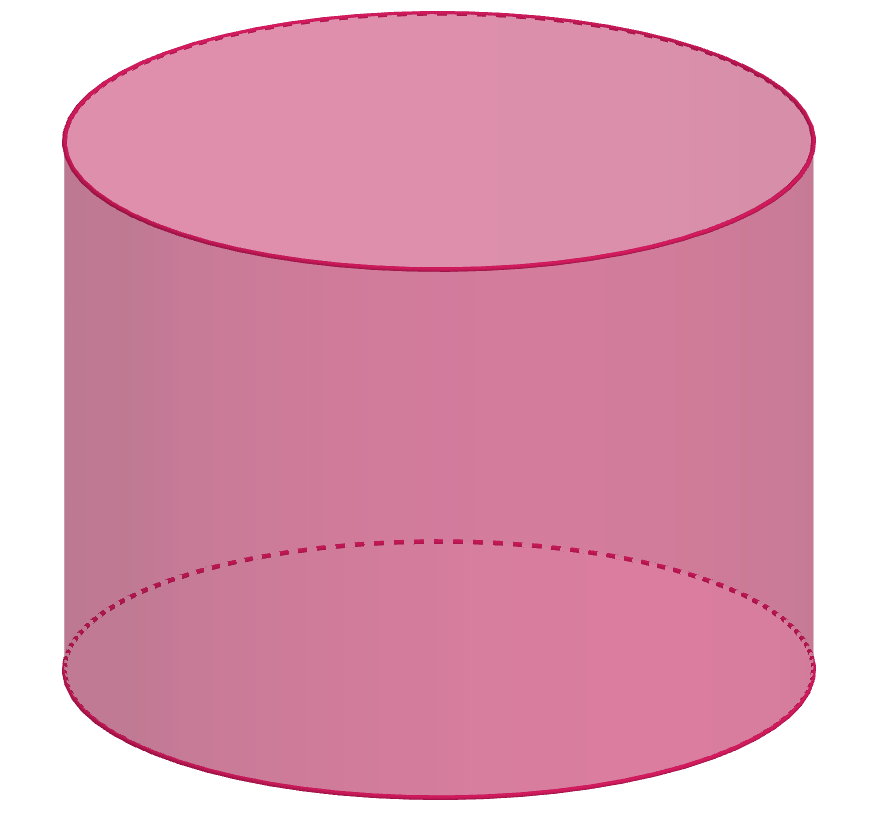
\includegraphics[width=0.5\columnwidth]{cylindre.png}
    \caption{Un cylindre, dans toute sa simplicité}
    \label{fig:cyl}
\end{figure}

\end{centering}

\subsection{Soluce}
On décompose notre cylindre en petit cylindre de hauteur $\intg z$ et additionne les volumes de tous ces cylindres pour trouver le volume du cylindre. Le volume de chacun de ces cylindres est $\pi r(z)^2 \intg y$. Il ne reste plus qu'à trouver $r(z)$.\newline
On connaît les équations du cylindre $x^2 + y^2 = R^2$ et $0\leq z \leq h$. Pour chacun de ces cylindres, on est dans un plan parallèle à $xOy$, c'est à dire qu'on est à $z$ fixé. On connaît l'équation d'un cercle dans un tel plan $x^2+y^2 = r(z)^2$, on en déduit que $x^2 + y^2 = R^2 = r(z)^2$. Donc, le volume du cylindre pour un $z$ donné est $\pi R^2 \intg z $, il ne reste plus qu'à sommer :
\begin{equation}
    V_{\mathrm{cyl}} = \displaystyle \int_{0}^{h} \pi R^2 \, \intg z = \pi R^2 h
\end{equation}

\section{La deuxième [2pt; 0.5pt pour la décompo en cylindre, 1pt pour avoir posé la bonne intégrale, 0.5 pour le résultat]}
Les toupies ne sont pas mal non plus. Celle-ci possède le petit désavantage d'être infinie. Mais son équation cartésienne est plutôt lisible :
\begin{equation*}
\left\{ 
        \begin{array}{rl}
    x^2+y^2&=\frac{1}{\sqrt{\abs{z}}}\\
    \abs{z}&\leq 5
    \end{array}
    \right.
\end{equation*}
Trouvez la valeur du volume de cette toupie (que vous pouvez admirer sur la figure \ref{fig:toup}) en utilisant une intégrale.

\subsection{Soluce}
On décompose la toupie en petit cylindre de hauteur $\intg z$ et on  additionne les volumes de tous ces cylindres pour trouver le volume de la toupie. Le volume de chacun des cylindres est $\pi r(z)^2 \intg y$.\newline
A $z$ fixé, on connaît l'équation d'un cercle dans le plan $xOy$: $x^2+y^2 = \frac{1}{\sqrt{\abs{z}}}$, on en déduit que $x^2 + y^2 =  \frac{1}{\sqrt{\abs{z}}} = r(z)^2$. Donc, le volume du cylindre pour un $z$ donné est $\pi  \frac{1}{\sqrt{\abs{z}}} \intg z $, il ne reste plus qu'à sommer :
\begin{equation}
    V_{\mathrm{toupie}} = \displaystyle \int_{-5}^{5} \pi  \frac{1}{\sqrt{\abs{z}}} \, \intg z = 2\displaystyle \int_{0}^{5} \pi  \frac{1}{\sqrt{z}} \, \intg z
\end{equation}
Qui est une intégrale généralisée. On trouve finalement
\begin{equation}
    V_{\mathrm{toupie}} = 2\pi\lim \limits_{\epsilon \rightarrow 0}\left[2\sqrt{z} \right]_\epsilon^5 = 4\pi\sqrt{5}
\end{equation}




\begin{centering}

\begin{figure}
    \centering
    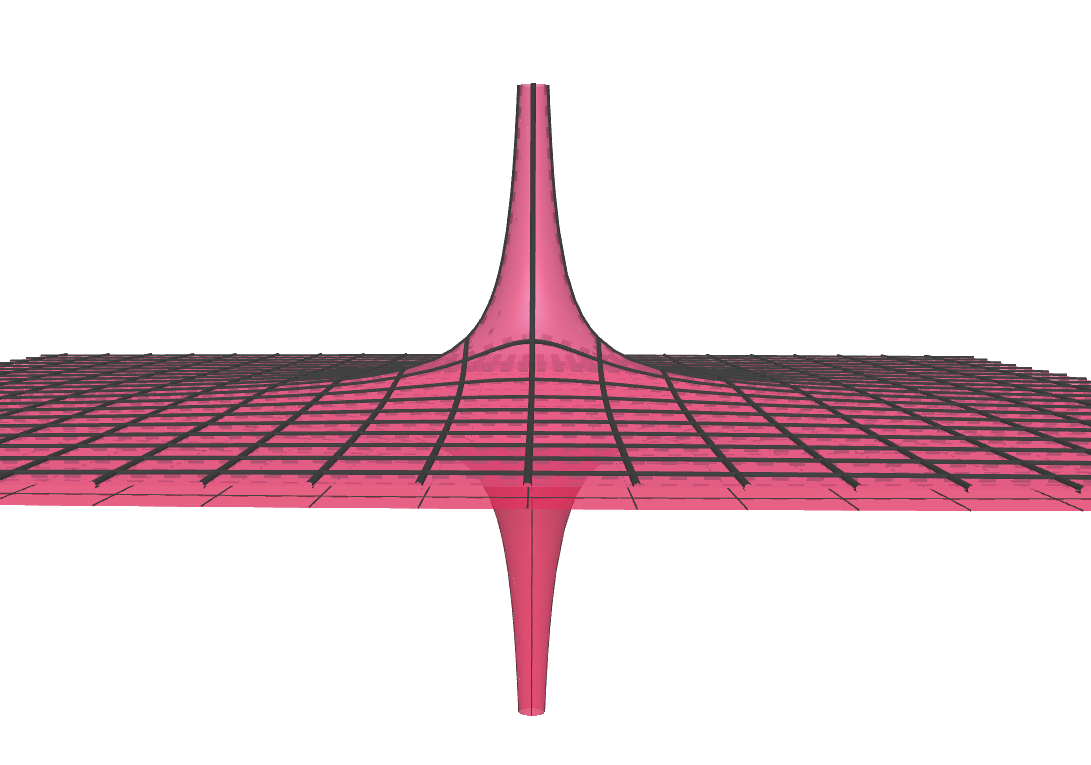
\includegraphics[width=0.5\columnwidth]{toupie}
    \caption{Une toupie, dans toute son infinité}
    \label{fig:toup}
\end{figure}



\end{centering}
\end{document}
